\begin{center}
	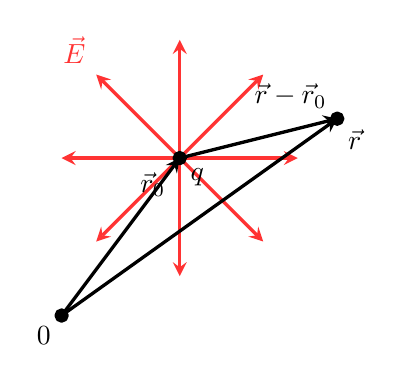
\begin{tikzpicture}[line width = 1.2pt, line join=round,x=1cm,y=1cm,>=stealth]
		% Koordinatensystem
		%\draw [->] (-2,0) -- (2,0) node[anchor=west] {$x$};
		%\draw [->] (0,-2) -- (0,2) node[anchor=south] {$y$};
		% elektrisches Feld
		\draw [<->,color=red!80] (-1.5,0) -- (1.5,0);
		\draw [<->,color=red!80] (0,-1.5) -- (0,1.5);
		\draw [<->,color=red!80] (-1.06066,-1.06066) -- (1.06066,1.06066);
		\draw [<->,color=red!80] (-1.06066,1.06066) -- (1.06066,-1.06066);
		\draw [color=red!80] (-1.06066,1.06066) node[anchor=south east]{$\vec{E}$};
		%\draw [color=red!40,style=dashed] (0,0) circle (1.5);
		% Aufpunkt
		\draw [->,color=black] (-1.5,-2) -- (2,0.5) node[anchor=north west]{$\vec{r} $};
		\draw [->,color=black] (-1.5,-2) -- (0,0) node[below left=1.3]{$\vec{r} _0$};
		\draw [->,color=black] (0,0) -- (2,0.5) node[above left=-0.1]{$\vec{r} -\vec{r} _0$};
		\filldraw [color=black] (2,0.5) circle (2pt);
		\filldraw [color=black] (-1.5,-2) circle (2pt);
		\draw [color=black] (-1.5,-2)  node[anchor=north east]{$0$};
		%\draw [color=black] (1.5,1.5) node[anchor=north east] {$\vec{r} $};
		% Ladung
		\filldraw [color=black] (0,0) circle (2pt);
		\draw [color=black] (0,0) node[anchor=north west]{$q$};
	\end{tikzpicture}
\end{center}
